\documentclass[12pt,english]{rftthesis}

\usepackage[utf8]{inputenc}
\usepackage[T1]{fontenc}
\usepackage{csquotes}
\usepackage{graphicx}
\usepackage{wrapfig}

\setacronymstyle{long-short}


\title           {Development of snapshot and fault injection techniques within Dream Chaser's COMS system's hypervisor}
\type            {Masters thesis abstract}
\author          {B.Eng. Alexis Cabana-Loriaux}
\matriculation   {0407200}
\studies         {Masters of Space Engineering}
\firstsupervisor {Prof. Dr.-Ing. Klaus Brieß}
\secondsupervisor{Dipl.-Ing. XXXX}
\industrysupervisor{Dipl.-Ing. Claudio Discepola}
\date            {\today}

\begin{document}


%
%  HEADER
%
\begin{center}
\begin{large}
Project description - Masters thesis
\end{large}
\\
\vspace{.5cm}
\begin{LARGE}
Development of Snapshot and Fault Injection Techniques within Dream Chaser's COMS System's Hypervisor
\end{LARGE}
\end{center}

%
%  Intro 
%
\section*{Introduction}\label{sec:intro}
The Dream Chaser Cargo System (DCCS) is a reusable orbital spaceplane from Sierra Nevada Corporation (SNC) intented for the resupply of both pressurized and unpressurized cargo to the International Space Station. The vehicle, whose development started in 2010, is to be launched on United Launch Alliance rockets, with the possibility of also serving european interests in space in the future. Since then, SNC has put MacDonald, Dettwiler and Associates Ltd. (MDA) in charge of the systems engineering and the development of the communication subsytem of DCCS. MDA is the industry supporter of the present thesis.

\begin{wrapfigure}{R}{0.45\textwidth}
\centering
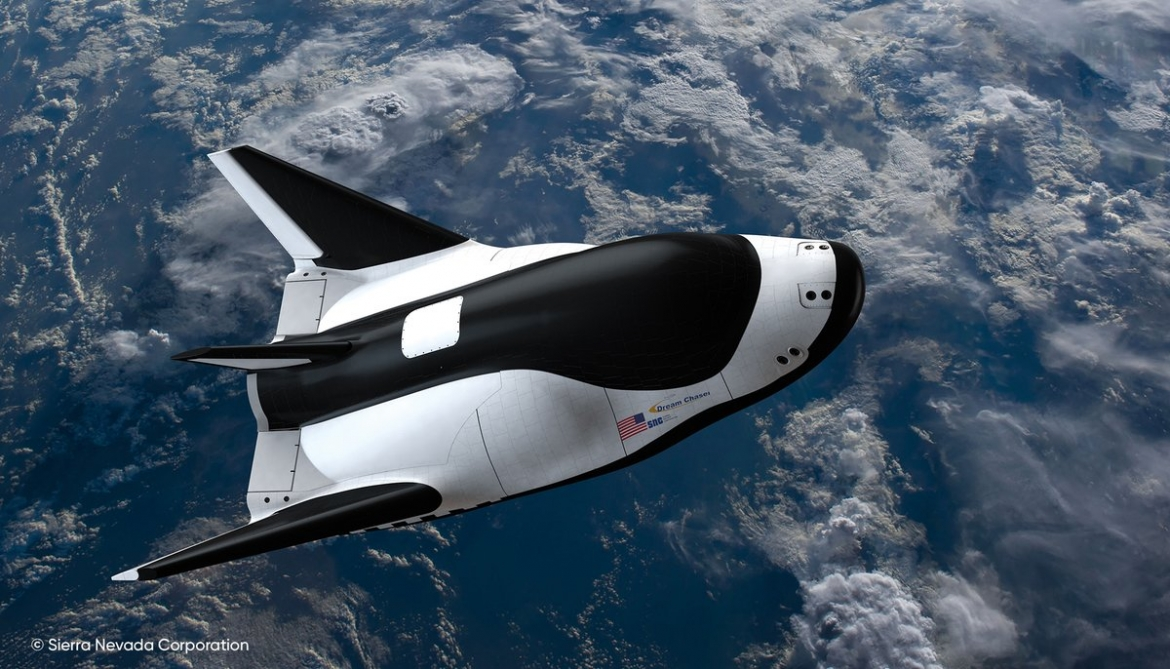
\includegraphics[width=0.4\textwidth]{art/dccs}
\caption{\label{fig:dccs}Artist impression of the Dream Chaser Cargo System. [Sierra Nevada Corporation]}
\end{wrapfigure}

With the ever decreasing cost of computing power, functional simulation of components and systems has become an integral part of the testing phase in space design. This approach is thus also taken by SNC, who requires their technology partners like MDA to provide simulators of their respective subsystems in order to mimic the behavior of some segments of the spacecraft in action together. As such, MDA is developing the Baseband Processor Simulator (BBPSim), a hypervisor that runs the COMS subsystem's software.

%
%  Purpose 
%
\section*{Purpose}\label{sec:purpose}

%
%  Tasks 
%
\section*{Summary of tasks}\label{sec:tasks}


\end{document}
